\chapter{Технологический раздел}
\label{cha:impl}

В данном разделе описываются технические средства,  используемые при проектировании распределенной системы обработки информации. Также приведены результаты разработки и тестирования системы. 

\section{Среда разработки, язык программирования}
Разработка распределенной системы осуществлялась на языке Java с использованием MVC библиотеки Play!
Язык Java был выбран, потому что он является переносимым и имеет обширную библиотеку стандартных функций, значительно ускоряющих разработку приложений. Фреймворк Play! был выбран, поскольку он содержит множество классов, помогающих в разработке Web-интерфейса участников и обмене сообщениями между ними. Среда IntelliJ IDEA была выбрана, так как является кроссплатформенной средой разработки, поддерживает выбранный фреймворк и бесплатна для использования в учебных целях.

\section{Выбор протоколов взаимодействия}

\subsection{Протокол асинхронного взаимодествия}

В качестве протокола асинхронного взаимодействия был выбран протокол SMTP, так как он является одним из рекомендуемых кафедрой протоколов для выполнения курсового проектирования.

\subsection{Протокол синхронного взаимодействия}

В качестве протокола синхронного взаимодействия был использован протокол HTTP/REST, так как он является наиболее удобным протоколом для реализации в MVC-фреймворке и позволяет унифицированно взаимодейтсвовать как пользователю с системой, так и системам между собой.

\section{Выбор формата передачи данных|

В качестве формата запроса для синхронного протокола был использован формат x-www-form-urlencoded, поскольку его можно использовать как на стороне клиента (HTML-формы и Javascript), так и на стороне сервера.
В качестве формата ответа для синхронного протокола, а также запроса для асинхронного протокола был использован JSON, поскольку он является одним из широкоиспользуемых текстовых форматов и имеет развитые библиотеки как на стороне клиента, так и на стороне сервера.

\section{Диаграммы классов}

\subsection{Исследующая система}
На рисунке ~\ref{fig:class-survey} показаны классы для системы исследующей организации, за исключением моделей и автоматически сгенерированных представлений.
\begin{figure}[ht]
  \centering
  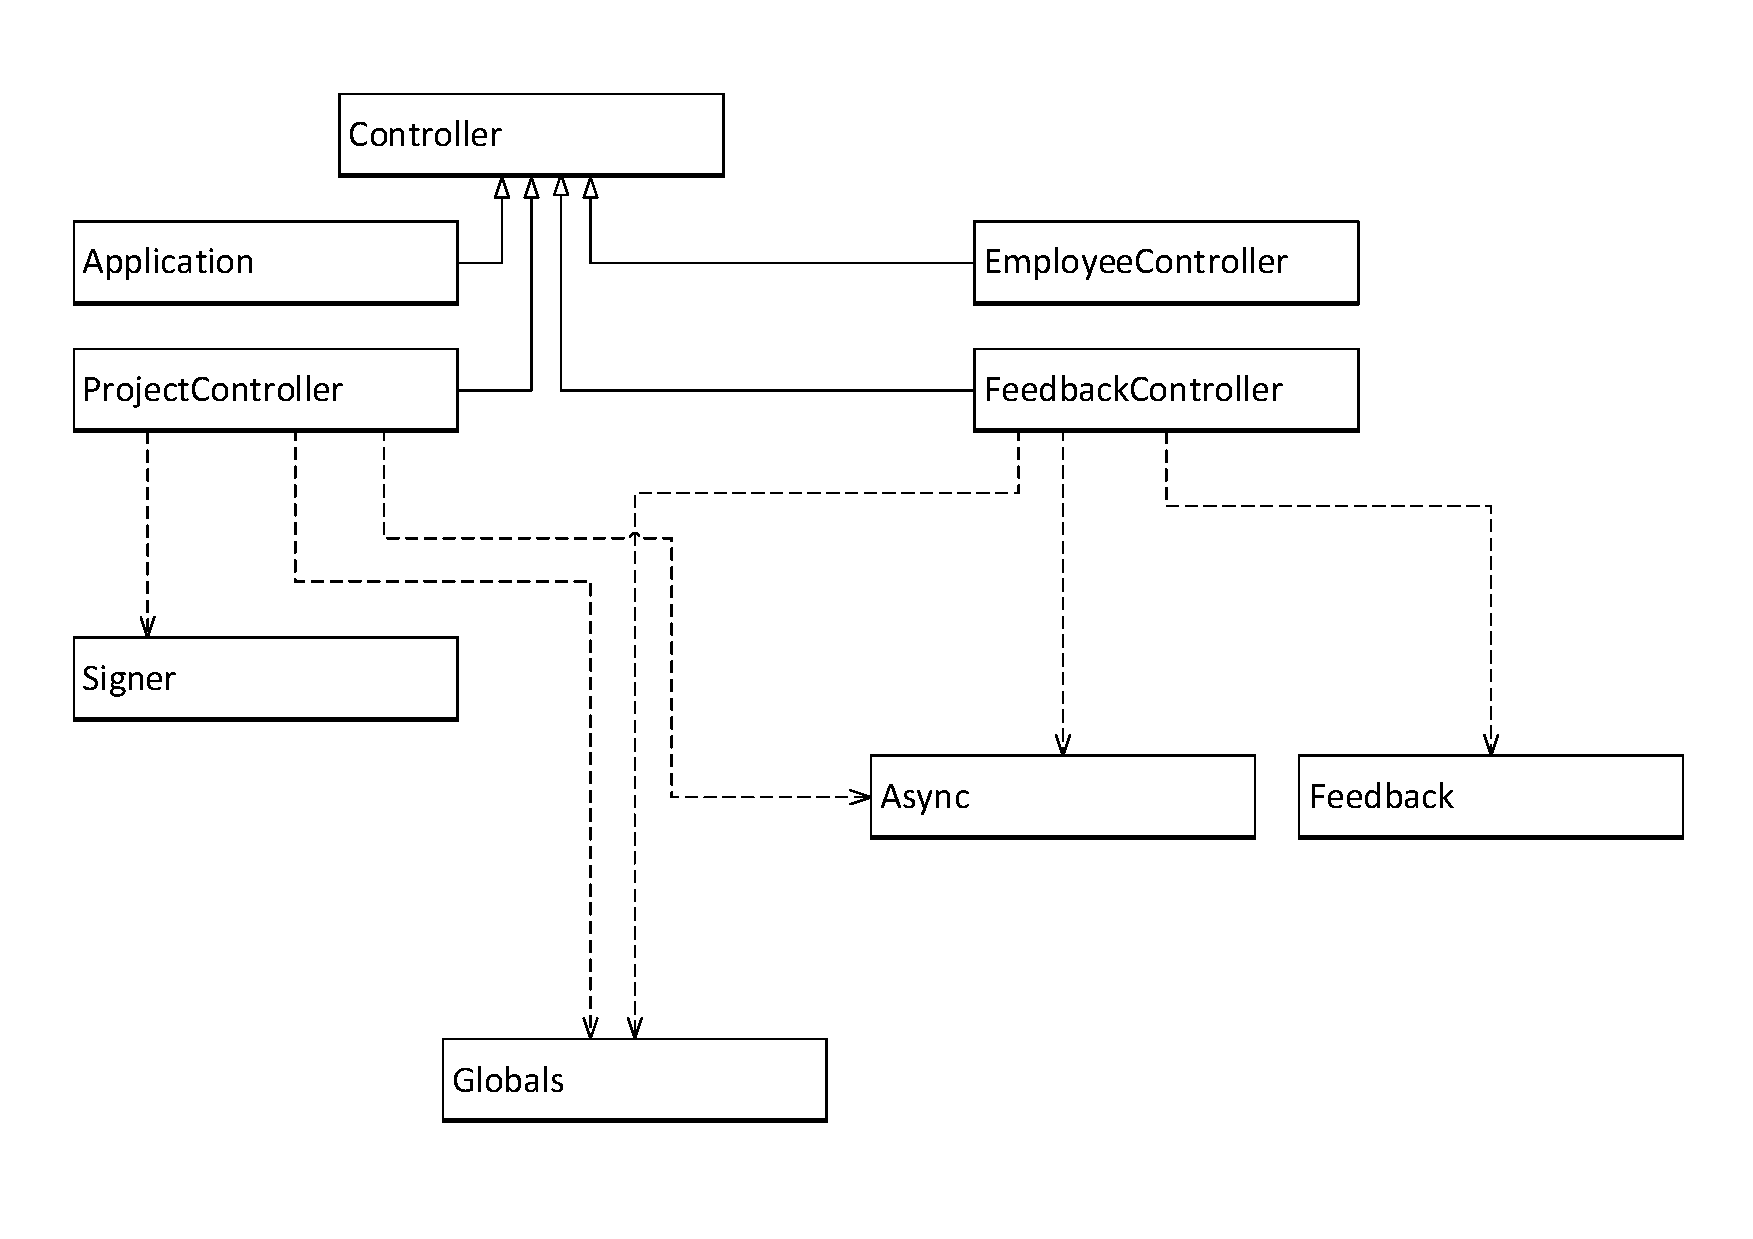
\includegraphics[width=\textwidth]{include/class-survey.pdf}
  \caption{Диаграмма классов исследующей системы}
  \label{fig:class-survey}
\end{figure}

\begin{enumerate}
\item Контроллеры:
\begin{enumerate}
\item Application - основной контроллер системы, реализующий функции авторизации через сервис Google.
\item EmployeeController - контроллер, осуществляющий добавление, редактирование и удаление респондентов.
\item ProjectController - контроллер, осуществляющий добавление и удалений проектов, создание и удалений вакансий в рекрутинговых агентствах и загрузку откликов.
\item FeedbackController - контроллер, осуществляющий кэширование данных о рекрутинговых агентствах, а также реализующий отправку отзыва об агентстве.
\end{enumerate}
\item Globals - модель, реализующая хранение системных переменных типа "ключ-значение". Используется для хранения времени последнего кэширования списка рекрутинговых агентств.
\item Async - класс, реализующий отправку асинхронных сообщений по протоколу SMTP.
\item Signer - класс, осуществляющий подпись синхронных и асинхронных запросов к рекрутинговым системам.
\item Feedback - класс, использующийся для промежуточного представления отзыва перед отправкой его контролирующей системе.
\end{enumerate}

\subsection{Контролирующая система}
На рисунке ~\ref{fig:class-supervising} показаны классы для системы контролирующей ассоциации, за исключением автоматически сгенерированных представлений.
\begin{figure}[ht]
  \centering
  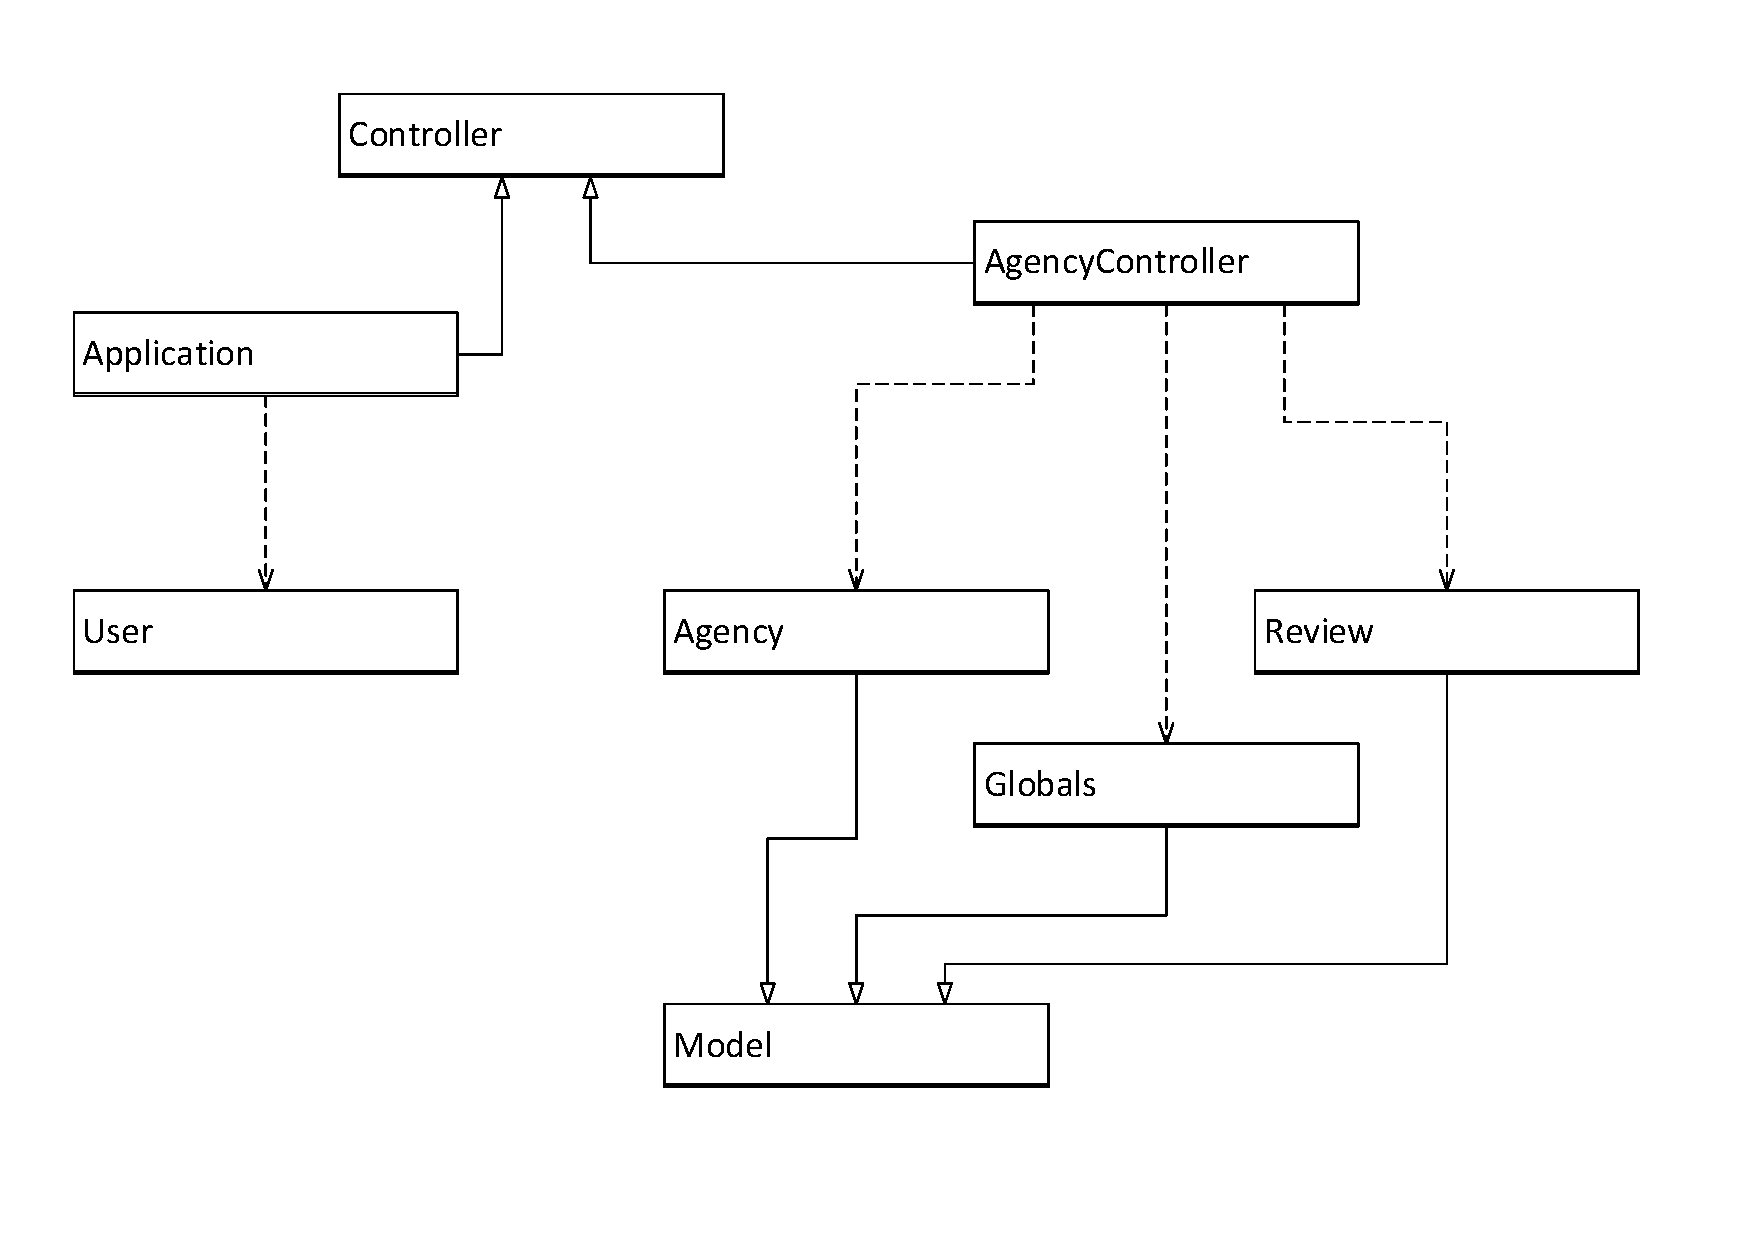
\includegraphics[width=\textwidth]{include/class-supervising.pdf}
  \caption{Диаграмма классов контролирующей системы}
  \label{fig:class-supervising}
\end{figure}

\begin{enumerate}
\item Контроллеры:
\begin{enumerate}
\item Application - основной контроллер системы, реализующий функции авторизации.
\item AgencyController - контроллер, реализующий добавление и удалений рекрутинговых агентств, а также получение отзывов о них.
\end{enumerate}
\item Модели:
\begin{enumerate}
\item Globals - модель, реализующая хранение системных переменных типа "ключ-значение". Используется для хранения последнего прочитанного сообщения POP3.
\item Review - модель, представляющая отзыв о рекрутинговом агентстве.
\item Agency - модель, представляющая рекрутингового агентство.
\end{enumerate}
\item User - класс, представляющий модель оператора контролирующей системы.
\end{enumerate}

\subsection{Рекрутинговая система}
На рисунке ~\ref{fig:class-recruiting} показаны классы для системы рекрутингового агентства, за исключением моделей и автоматически сгенерированных представлений.
\begin{figure}[ht]
  \centering
  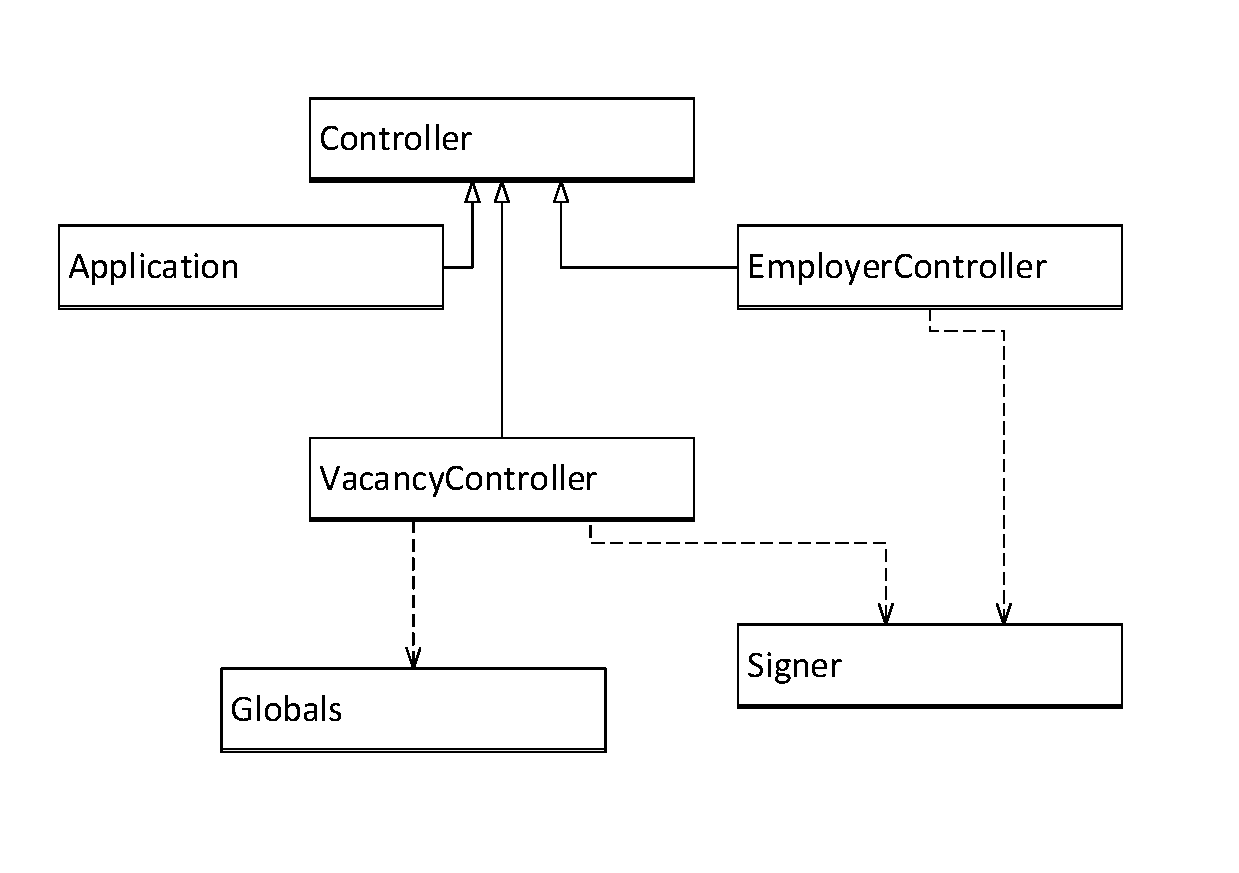
\includegraphics[width=\textwidth]{include/class-recruiting.pdf}
  \caption{Диаграмма классов рекрутинговой системы}
  \label{fig:class-recruiting}
\end{figure}

\begin{enumerate}
\item Контроллеры:
\begin{enumerate}
\item Application - основной контроллер системы, реализующий функции авторизации и регистрации.
\item EmployerController - контроллер, реализующий добавление и удалений работодателей и их секретных ключей.
\item VacancyController - контроллер, реализующий прием заявок на создание и удаление вакансий.
\end{enumerate}
\item Globals - модель, реализующая хранение системных переменных типа "ключ-значение". Используется для хранения последнего прочитанного сообщения POP3.
\item Signer - класс, осуществляющий проверку подписи синхронных и асинхронных запросов.
\end{enumerate}

\section{Реализация цифровой подписи}
В качестве алгоритма цифровой подписи использован алгоритм, аналогичный тому, что применяется в протоколе OAuth. В качестве алгоритма шифрования для подписи использовался HMAC с хэш-функцией SHA256. Шаги составления подписи:
\begin{enumerate}
\item Для подписанных запросов добавляется параметр time, представляющий unix-time.
\item Формируется строка для подписи, представляющая из себя целевой URL, знак ? (вопроса), затем параметры запроса в виде ключ=значение, отсортированные по алфавиту по ключу и разделенные знаком & (амперсанд). Для асинхронного запроса целевой URL и знак вопроса опускаются.
\item Формируется подпись - зашифрованная выбранным алгоритмом строка с использованием секретного ключа.
\item Далее подпись добавляется как параметр signature к остальным параметрам запроса.

Для проверки подписи на принимающей стороне используется аналогичный алгоритм. Для выбора ключа запрос должен содержать email отправителя. Параметр signature не участвует в создании строки для подписи.

%%% Local Variables:
%%% mode: latex
%%% TeX-master: "rpz"
%%% End:
